\documentclass[twoside]{book}

% Packages required by doxygen
\usepackage{fixltx2e}
\usepackage{calc}
\usepackage{doxygen}
\usepackage[export]{adjustbox} % also loads graphicx
\usepackage{graphicx}
\usepackage[utf8]{inputenc}
\usepackage{makeidx}
\usepackage{multicol}
\usepackage{multirow}
\PassOptionsToPackage{warn}{textcomp}
\usepackage{textcomp}
\usepackage[nointegrals]{wasysym}
\usepackage[table]{xcolor}

% Font selection
\usepackage[T1]{fontenc}
\usepackage[scaled=.90]{helvet}
\usepackage{courier}
\usepackage{amssymb}
\usepackage{sectsty}
\renewcommand{\familydefault}{\sfdefault}
\allsectionsfont{%
  \fontseries{bc}\selectfont%
  \color{darkgray}%
}
\renewcommand{\DoxyLabelFont}{%
  \fontseries{bc}\selectfont%
  \color{darkgray}%
}
\newcommand{\+}{\discretionary{\mbox{\scriptsize$\hookleftarrow$}}{}{}}

% Page & text layout
\usepackage{geometry}
\geometry{%
  a4paper,%
  top=2.5cm,%
  bottom=2.5cm,%
  left=2.5cm,%
  right=2.5cm%
}
\tolerance=750
\hfuzz=15pt
\hbadness=750
\setlength{\emergencystretch}{15pt}
\setlength{\parindent}{0cm}
\setlength{\parskip}{3ex plus 2ex minus 2ex}
\makeatletter
\renewcommand{\paragraph}{%
  \@startsection{paragraph}{4}{0ex}{-1.0ex}{1.0ex}{%
    \normalfont\normalsize\bfseries\SS@parafont%
  }%
}
\renewcommand{\subparagraph}{%
  \@startsection{subparagraph}{5}{0ex}{-1.0ex}{1.0ex}{%
    \normalfont\normalsize\bfseries\SS@subparafont%
  }%
}
\makeatother

% Headers & footers
\usepackage{fancyhdr}
\pagestyle{fancyplain}
\fancyhead[LE]{\fancyplain{}{\bfseries\thepage}}
\fancyhead[CE]{\fancyplain{}{}}
\fancyhead[RE]{\fancyplain{}{\bfseries\leftmark}}
\fancyhead[LO]{\fancyplain{}{\bfseries\rightmark}}
\fancyhead[CO]{\fancyplain{}{}}
\fancyhead[RO]{\fancyplain{}{\bfseries\thepage}}
\fancyfoot[LE]{\fancyplain{}{}}
\fancyfoot[CE]{\fancyplain{}{}}
\fancyfoot[RE]{\fancyplain{}{\bfseries\scriptsize Generated by Doxygen }}
\fancyfoot[LO]{\fancyplain{}{\bfseries\scriptsize Generated by Doxygen }}
\fancyfoot[CO]{\fancyplain{}{}}
\fancyfoot[RO]{\fancyplain{}{}}
\renewcommand{\footrulewidth}{0.4pt}
\renewcommand{\chaptermark}[1]{%
  \markboth{#1}{}%
}
\renewcommand{\sectionmark}[1]{%
  \markright{\thesection\ #1}%
}

% Indices & bibliography
\usepackage{natbib}
\usepackage[titles]{tocloft}
\setcounter{tocdepth}{3}
\setcounter{secnumdepth}{5}
\makeindex

% Hyperlinks (required, but should be loaded last)
\usepackage{ifpdf}
\ifpdf
  \usepackage[pdftex,pagebackref=true]{hyperref}
\else
  \usepackage[ps2pdf,pagebackref=true]{hyperref}
\fi
\hypersetup{%
  colorlinks=true,%
  linkcolor=blue,%
  citecolor=blue,%
  unicode%
}

% Custom commands
\newcommand{\clearemptydoublepage}{%
  \newpage{\pagestyle{empty}\cleardoublepage}%
}

\usepackage{caption}
\captionsetup{labelsep=space,justification=centering,font={bf},singlelinecheck=off,skip=4pt,position=top}

%===== C O N T E N T S =====

\begin{document}

% Titlepage & ToC
\hypersetup{pageanchor=false,
             bookmarksnumbered=true,
             pdfencoding=unicode
            }
\pagenumbering{alph}
\begin{titlepage}
\vspace*{7cm}
\begin{center}%
{\Large C\+P\+U\+Information1 }\\
\vspace*{1cm}
{\large Generated by Doxygen 1.8.13}\\
\end{center}
\end{titlepage}
\clearemptydoublepage
\pagenumbering{roman}
\tableofcontents
\clearemptydoublepage
\pagenumbering{arabic}
\hypersetup{pageanchor=true}

%--- Begin generated contents ---
\chapter{Hierarchical Index}
\section{Class Hierarchy}
This inheritance list is sorted roughly, but not completely, alphabetically\+:\begin{DoxyCompactList}
\item Q\+Object\begin{DoxyCompactList}
\item \contentsline{section}{C\+P\+U\+Info}{\pageref{class_c_p_u_info}}{}
\item \contentsline{section}{C\+P\+U\+List}{\pageref{class_c_p_u_list}}{}
\item \contentsline{section}{File\+Manager}{\pageref{class_file_manager}}{}
\item \contentsline{section}{Info\+Manager}{\pageref{class_info_manager}}{}
\end{DoxyCompactList}
\end{DoxyCompactList}

\chapter{Class Index}
\section{Class List}
Here are the classes, structs, unions and interfaces with brief descriptions\+:\begin{DoxyCompactList}
\item\contentsline{section}{\hyperlink{class_c_p_u_info}{C\+P\+U\+Info} }{\pageref{class_c_p_u_info}}{}
\item\contentsline{section}{\hyperlink{class_c_p_u_list}{C\+P\+U\+List} }{\pageref{class_c_p_u_list}}{}
\item\contentsline{section}{\hyperlink{class_file_manager}{File\+Manager} }{\pageref{class_file_manager}}{}
\item\contentsline{section}{\hyperlink{class_info_manager}{Info\+Manager} }{\pageref{class_info_manager}}{}
\end{DoxyCompactList}

\chapter{File Index}
\section{File List}
Here is a list of all files with brief descriptions\+:\begin{DoxyCompactList}
\item\contentsline{section}{C\+:/\+Users/\+S\+H\+E\+K\+H\+A\+R/\+Desktop/\+C\+P\+U\+\_\+\+Info/\+C\+P\+U\+Information1/\hyperlink{constantslist_8h}{constantslist.\+h} }{\pageref{constantslist_8h}}{}
\item\contentsline{section}{C\+:/\+Users/\+S\+H\+E\+K\+H\+A\+R/\+Desktop/\+C\+P\+U\+\_\+\+Info/\+C\+P\+U\+Information1/\hyperlink{cpuinfo_8cpp}{cpuinfo.\+cpp} }{\pageref{cpuinfo_8cpp}}{}
\item\contentsline{section}{C\+:/\+Users/\+S\+H\+E\+K\+H\+A\+R/\+Desktop/\+C\+P\+U\+\_\+\+Info/\+C\+P\+U\+Information1/\hyperlink{cpuinfo_8h}{cpuinfo.\+h} }{\pageref{cpuinfo_8h}}{}
\item\contentsline{section}{C\+:/\+Users/\+S\+H\+E\+K\+H\+A\+R/\+Desktop/\+C\+P\+U\+\_\+\+Info/\+C\+P\+U\+Information1/\hyperlink{cpulist_8cpp}{cpulist.\+cpp} }{\pageref{cpulist_8cpp}}{}
\item\contentsline{section}{C\+:/\+Users/\+S\+H\+E\+K\+H\+A\+R/\+Desktop/\+C\+P\+U\+\_\+\+Info/\+C\+P\+U\+Information1/\hyperlink{cpulist_8h}{cpulist.\+h} }{\pageref{cpulist_8h}}{}
\item\contentsline{section}{C\+:/\+Users/\+S\+H\+E\+K\+H\+A\+R/\+Desktop/\+C\+P\+U\+\_\+\+Info/\+C\+P\+U\+Information1/\hyperlink{filemanager_8cpp}{filemanager.\+cpp} }{\pageref{filemanager_8cpp}}{}
\item\contentsline{section}{C\+:/\+Users/\+S\+H\+E\+K\+H\+A\+R/\+Desktop/\+C\+P\+U\+\_\+\+Info/\+C\+P\+U\+Information1/\hyperlink{filemanager_8h}{filemanager.\+h} }{\pageref{filemanager_8h}}{}
\item\contentsline{section}{C\+:/\+Users/\+S\+H\+E\+K\+H\+A\+R/\+Desktop/\+C\+P\+U\+\_\+\+Info/\+C\+P\+U\+Information1/\hyperlink{infomanager_8cpp}{infomanager.\+cpp} }{\pageref{infomanager_8cpp}}{}
\item\contentsline{section}{C\+:/\+Users/\+S\+H\+E\+K\+H\+A\+R/\+Desktop/\+C\+P\+U\+\_\+\+Info/\+C\+P\+U\+Information1/\hyperlink{infomanager_8h}{infomanager.\+h} }{\pageref{infomanager_8h}}{}
\item\contentsline{section}{C\+:/\+Users/\+S\+H\+E\+K\+H\+A\+R/\+Desktop/\+C\+P\+U\+\_\+\+Info/\+C\+P\+U\+Information1/\hyperlink{main_8cpp}{main.\+cpp} }{\pageref{main_8cpp}}{}
\end{DoxyCompactList}

\chapter{Class Documentation}
\hypertarget{class_c_p_u_info}{}\section{C\+P\+U\+Info Class Reference}
\label{class_c_p_u_info}\index{C\+P\+U\+Info@{C\+P\+U\+Info}}


{\ttfamily \#include $<$cpuinfo.\+h$>$}

Inheritance diagram for C\+P\+U\+Info\+:\begin{figure}[H]
\begin{center}
\leavevmode
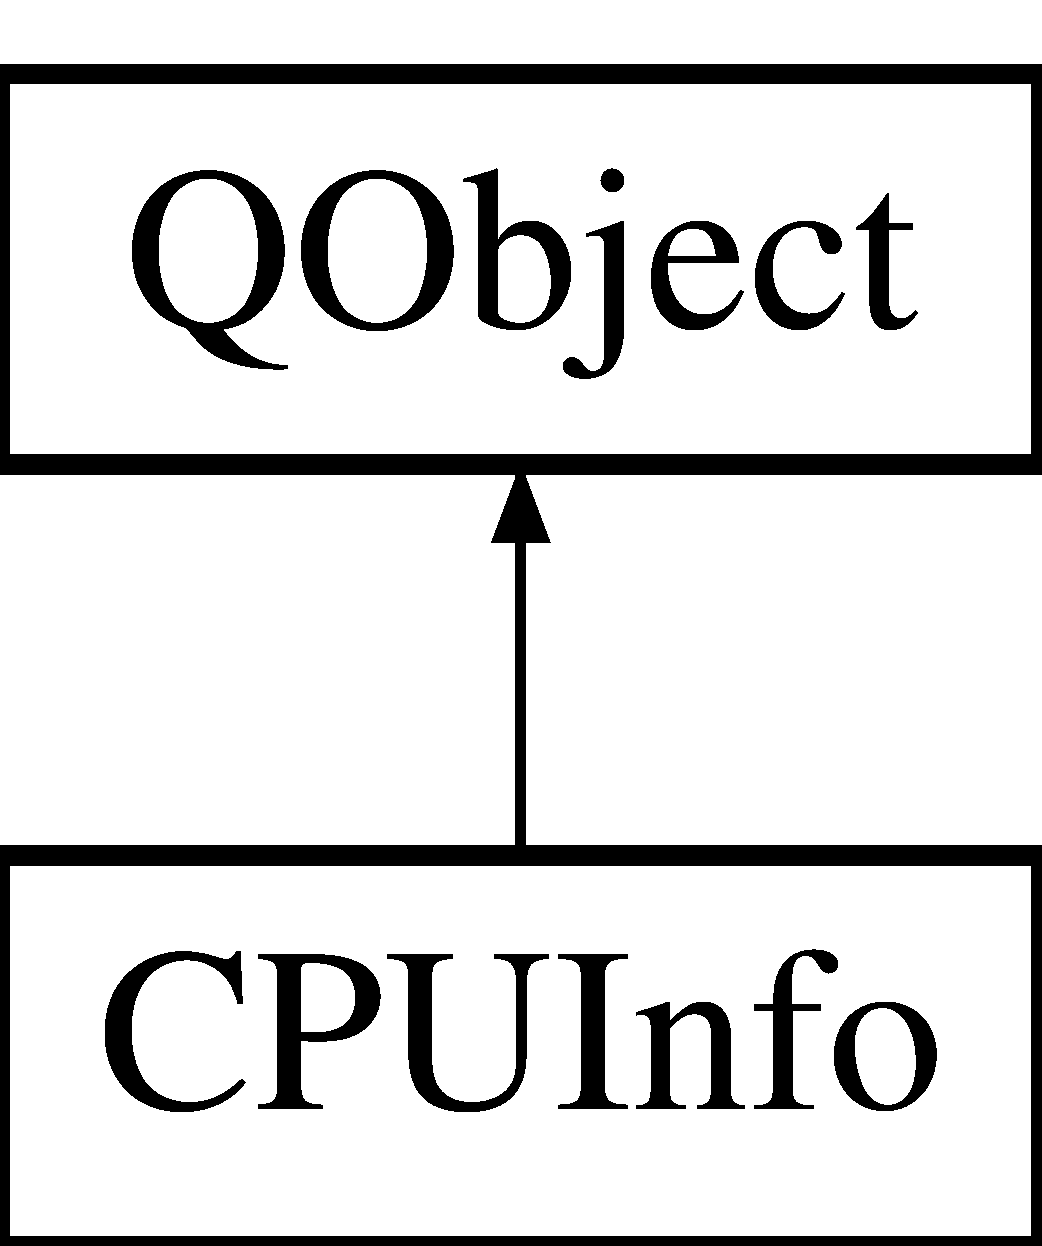
\includegraphics[height=2.000000cm]{class_c_p_u_info}
\end{center}
\end{figure}
\subsection*{Signals}
\begin{DoxyCompactItemize}
\item 
void \hyperlink{class_c_p_u_info_a3b989dd75a0c8fc1f1317f9695ef6ae0}{processor\+Id\+\_\+changed} ()
\item 
void \hyperlink{class_c_p_u_info_aa4908f61258f88c4330f665061941354}{cpu\+Frequency\+\_\+changed} ()
\end{DoxyCompactItemize}
\subsection*{Public Member Functions}
\begin{DoxyCompactItemize}
\item 
\hyperlink{class_c_p_u_info_ae64d136af2ac562ebad60497c9c20afa}{C\+P\+U\+Info} (Q\+Object $\ast$parent=0)
\item 
Q\+String \hyperlink{class_c_p_u_info_a81e583c0d1a182dcf29243a7b6c2ae25}{processor\+Id} () const
\item 
void \hyperlink{class_c_p_u_info_af3b55c258009a1f81ff4367fce1e25a9}{set\+Processor\+Id} (const Q\+String \&\hyperlink{class_c_p_u_info_a63925ca12a5c5841a265566132461efc}{processor\+Id})
\item 
Q\+String \hyperlink{class_c_p_u_info_a5d8ffb64c8cca2b5867a4a460a0179ae}{cpu\+Frequency} () const
\item 
void \hyperlink{class_c_p_u_info_aa6607cae8f23ea68bd0a3c72cd4affda}{set\+Cpu\+Frequency} (const Q\+String \&\hyperlink{class_c_p_u_info_a08eacbffc7b4726058d011b966cd05b5}{cpu\+Frequency\+M\+Hz})
\end{DoxyCompactItemize}
\subsection*{Properties}
\begin{DoxyCompactItemize}
\item 
Q\+String \hyperlink{class_c_p_u_info_a63925ca12a5c5841a265566132461efc}{processor\+Id}
\item 
Q\+String \hyperlink{class_c_p_u_info_a08eacbffc7b4726058d011b966cd05b5}{cpu\+Frequency\+M\+Hz}
\end{DoxyCompactItemize}


\subsection{Constructor \& Destructor Documentation}
\mbox{\Hypertarget{class_c_p_u_info_ae64d136af2ac562ebad60497c9c20afa}\label{class_c_p_u_info_ae64d136af2ac562ebad60497c9c20afa}} 
\index{C\+P\+U\+Info@{C\+P\+U\+Info}!C\+P\+U\+Info@{C\+P\+U\+Info}}
\index{C\+P\+U\+Info@{C\+P\+U\+Info}!C\+P\+U\+Info@{C\+P\+U\+Info}}
\subsubsection{\texorpdfstring{C\+P\+U\+Info()}{CPUInfo()}}
{\footnotesize\ttfamily C\+P\+U\+Info\+::\+C\+P\+U\+Info (\begin{DoxyParamCaption}\item[{Q\+Object $\ast$}]{parent = {\ttfamily 0} }\end{DoxyParamCaption})\hspace{0.3cm}{\ttfamily [explicit]}}



\subsection{Member Function Documentation}
\mbox{\Hypertarget{class_c_p_u_info_a5d8ffb64c8cca2b5867a4a460a0179ae}\label{class_c_p_u_info_a5d8ffb64c8cca2b5867a4a460a0179ae}} 
\index{C\+P\+U\+Info@{C\+P\+U\+Info}!cpu\+Frequency@{cpu\+Frequency}}
\index{cpu\+Frequency@{cpu\+Frequency}!C\+P\+U\+Info@{C\+P\+U\+Info}}
\subsubsection{\texorpdfstring{cpu\+Frequency()}{cpuFrequency()}}
{\footnotesize\ttfamily Q\+String C\+P\+U\+Info\+::cpu\+Frequency (\begin{DoxyParamCaption}{ }\end{DoxyParamCaption}) const}

\mbox{\Hypertarget{class_c_p_u_info_aa4908f61258f88c4330f665061941354}\label{class_c_p_u_info_aa4908f61258f88c4330f665061941354}} 
\index{C\+P\+U\+Info@{C\+P\+U\+Info}!cpu\+Frequency\+\_\+changed@{cpu\+Frequency\+\_\+changed}}
\index{cpu\+Frequency\+\_\+changed@{cpu\+Frequency\+\_\+changed}!C\+P\+U\+Info@{C\+P\+U\+Info}}
\subsubsection{\texorpdfstring{cpu\+Frequency\+\_\+changed}{cpuFrequency\_changed}}
{\footnotesize\ttfamily void C\+P\+U\+Info\+::cpu\+Frequency\+\_\+changed (\begin{DoxyParamCaption}{ }\end{DoxyParamCaption})\hspace{0.3cm}{\ttfamily [signal]}}

\mbox{\Hypertarget{class_c_p_u_info_a81e583c0d1a182dcf29243a7b6c2ae25}\label{class_c_p_u_info_a81e583c0d1a182dcf29243a7b6c2ae25}} 
\index{C\+P\+U\+Info@{C\+P\+U\+Info}!processor\+Id@{processor\+Id}}
\index{processor\+Id@{processor\+Id}!C\+P\+U\+Info@{C\+P\+U\+Info}}
\subsubsection{\texorpdfstring{processor\+Id()}{processorId()}}
{\footnotesize\ttfamily Q\+String C\+P\+U\+Info\+::processor\+Id (\begin{DoxyParamCaption}{ }\end{DoxyParamCaption}) const}

\mbox{\Hypertarget{class_c_p_u_info_a3b989dd75a0c8fc1f1317f9695ef6ae0}\label{class_c_p_u_info_a3b989dd75a0c8fc1f1317f9695ef6ae0}} 
\index{C\+P\+U\+Info@{C\+P\+U\+Info}!processor\+Id\+\_\+changed@{processor\+Id\+\_\+changed}}
\index{processor\+Id\+\_\+changed@{processor\+Id\+\_\+changed}!C\+P\+U\+Info@{C\+P\+U\+Info}}
\subsubsection{\texorpdfstring{processor\+Id\+\_\+changed}{processorId\_changed}}
{\footnotesize\ttfamily void C\+P\+U\+Info\+::processor\+Id\+\_\+changed (\begin{DoxyParamCaption}{ }\end{DoxyParamCaption})\hspace{0.3cm}{\ttfamily [signal]}}

\mbox{\Hypertarget{class_c_p_u_info_aa6607cae8f23ea68bd0a3c72cd4affda}\label{class_c_p_u_info_aa6607cae8f23ea68bd0a3c72cd4affda}} 
\index{C\+P\+U\+Info@{C\+P\+U\+Info}!set\+Cpu\+Frequency@{set\+Cpu\+Frequency}}
\index{set\+Cpu\+Frequency@{set\+Cpu\+Frequency}!C\+P\+U\+Info@{C\+P\+U\+Info}}
\subsubsection{\texorpdfstring{set\+Cpu\+Frequency()}{setCpuFrequency()}}
{\footnotesize\ttfamily void C\+P\+U\+Info\+::set\+Cpu\+Frequency (\begin{DoxyParamCaption}\item[{const Q\+String \&}]{cpu\+Frequency\+M\+Hz }\end{DoxyParamCaption})}

\mbox{\Hypertarget{class_c_p_u_info_af3b55c258009a1f81ff4367fce1e25a9}\label{class_c_p_u_info_af3b55c258009a1f81ff4367fce1e25a9}} 
\index{C\+P\+U\+Info@{C\+P\+U\+Info}!set\+Processor\+Id@{set\+Processor\+Id}}
\index{set\+Processor\+Id@{set\+Processor\+Id}!C\+P\+U\+Info@{C\+P\+U\+Info}}
\subsubsection{\texorpdfstring{set\+Processor\+Id()}{setProcessorId()}}
{\footnotesize\ttfamily void C\+P\+U\+Info\+::set\+Processor\+Id (\begin{DoxyParamCaption}\item[{const Q\+String \&}]{processor\+Id }\end{DoxyParamCaption})}



\subsection{Property Documentation}
\mbox{\Hypertarget{class_c_p_u_info_a08eacbffc7b4726058d011b966cd05b5}\label{class_c_p_u_info_a08eacbffc7b4726058d011b966cd05b5}} 
\index{C\+P\+U\+Info@{C\+P\+U\+Info}!cpu\+Frequency\+M\+Hz@{cpu\+Frequency\+M\+Hz}}
\index{cpu\+Frequency\+M\+Hz@{cpu\+Frequency\+M\+Hz}!C\+P\+U\+Info@{C\+P\+U\+Info}}
\subsubsection{\texorpdfstring{cpu\+Frequency\+M\+Hz}{cpuFrequencyMHz}}
{\footnotesize\ttfamily Q\+String C\+P\+U\+Info\+::cpu\+Frequency\+M\+Hz\hspace{0.3cm}{\ttfamily [read]}}

\mbox{\Hypertarget{class_c_p_u_info_a63925ca12a5c5841a265566132461efc}\label{class_c_p_u_info_a63925ca12a5c5841a265566132461efc}} 
\index{C\+P\+U\+Info@{C\+P\+U\+Info}!processor\+Id@{processor\+Id}}
\index{processor\+Id@{processor\+Id}!C\+P\+U\+Info@{C\+P\+U\+Info}}
\subsubsection{\texorpdfstring{processor\+Id}{processorId}}
{\footnotesize\ttfamily Q\+String C\+P\+U\+Info\+::processor\+Id\hspace{0.3cm}{\ttfamily [read]}, {\ttfamily [write]}}



The documentation for this class was generated from the following files\+:\begin{DoxyCompactItemize}
\item 
C\+:/\+Users/\+S\+H\+E\+K\+H\+A\+R/\+Desktop/\+C\+P\+U\+\_\+\+Info/\+C\+P\+U\+Information1/\hyperlink{cpuinfo_8h}{cpuinfo.\+h}\item 
C\+:/\+Users/\+S\+H\+E\+K\+H\+A\+R/\+Desktop/\+C\+P\+U\+\_\+\+Info/\+C\+P\+U\+Information1/\hyperlink{cpuinfo_8cpp}{cpuinfo.\+cpp}\end{DoxyCompactItemize}

\hypertarget{class_c_p_u_list}{}\section{C\+P\+U\+List Class Reference}
\label{class_c_p_u_list}\index{C\+P\+U\+List@{C\+P\+U\+List}}


{\ttfamily \#include $<$cpulist.\+h$>$}

Inheritance diagram for C\+P\+U\+List\+:\begin{figure}[H]
\begin{center}
\leavevmode
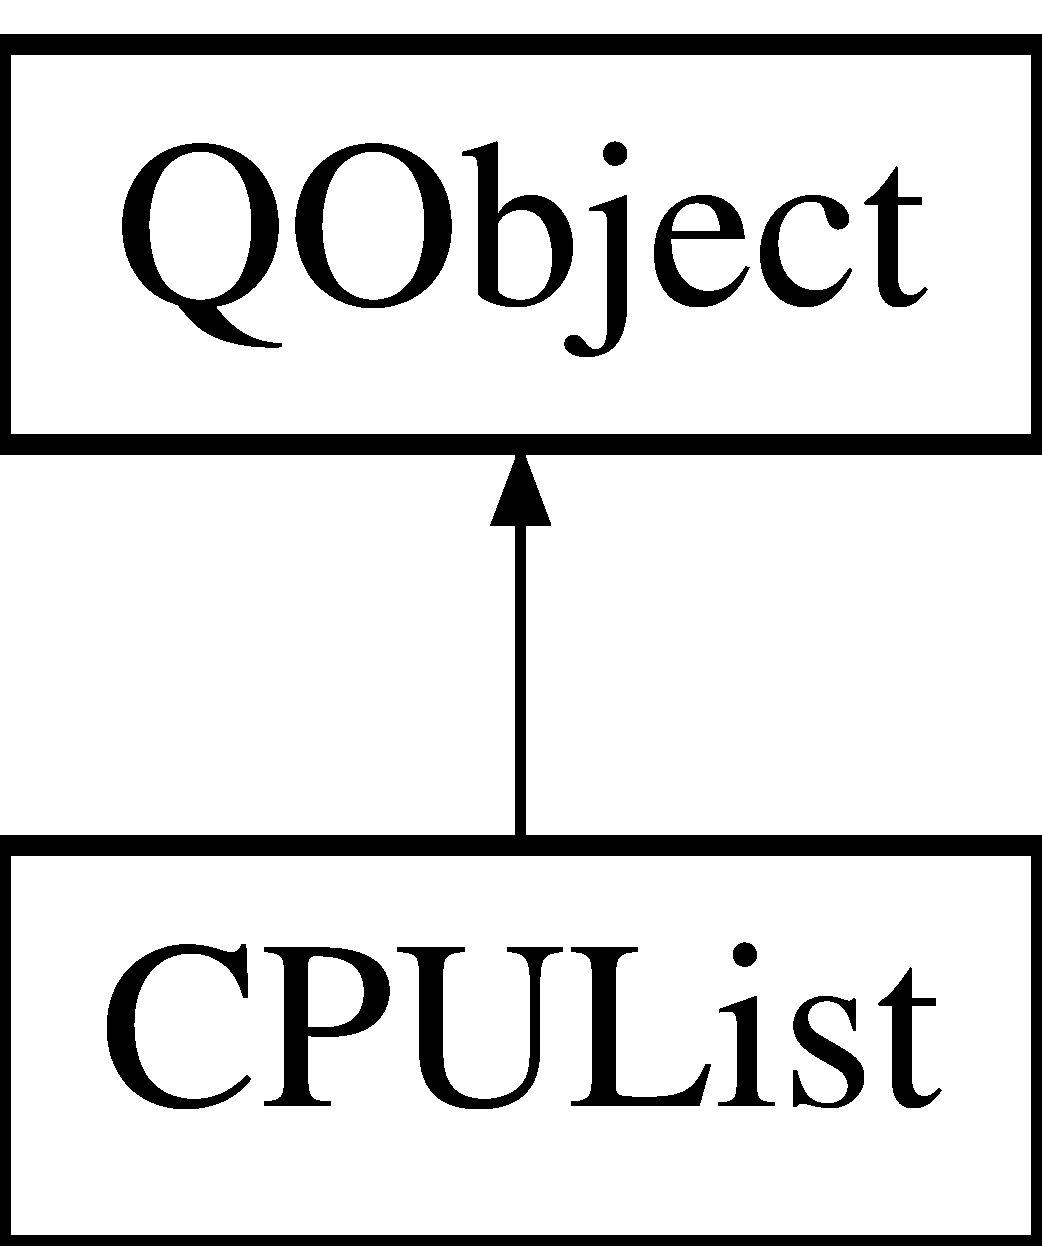
\includegraphics[height=2.000000cm]{class_c_p_u_list}
\end{center}
\end{figure}
\subsection*{Public Member Functions}
\begin{DoxyCompactItemize}
\item 
\hyperlink{class_c_p_u_list_af8d85299bb17bcd5f1989a907337c0d9}{C\+P\+U\+List} (Q\+Object $\ast$parent=0)
\item 
\hyperlink{class_c_p_u_list_a78f76d52368f52ca8466a7ed1f1a05b4}{$\sim$\+C\+P\+U\+List} ()
\item 
void \hyperlink{class_c_p_u_list_a9423eef0f279d40de6674857ded63907}{set\+C\+P\+U\+List} (Q\+List$<$ \hyperlink{class_c_p_u_info}{C\+P\+U\+Info} $\ast$$>$ list)
\item 
Q\+Qml\+List\+Property$<$ \hyperlink{class_c_p_u_info}{C\+P\+U\+Info} $>$ \hyperlink{class_c_p_u_list_a6d135eed8d40bfbb913e24848093f3ee}{get\+Processor\+List} ()
\item 
int \hyperlink{class_c_p_u_list_af608bafb0800d5bf5feb9bb2c008f1a9}{get\+Processor\+Count} () const
\item 
\hyperlink{class_c_p_u_info}{C\+P\+U\+Info} $\ast$ \hyperlink{class_c_p_u_list_a89903282b11ae6199d18907b0a4e6af3}{get\+C\+P\+U\+Info\+At} (int index) const
\item 
Q\+String \hyperlink{class_c_p_u_list_a0c172aa998f014f8b01e4a9fd79bb57a}{get\+Count} ()
\end{DoxyCompactItemize}
\subsection*{Properties}
\begin{DoxyCompactItemize}
\item 
Q\+Qml\+List\+Property$<$ \hyperlink{class_c_p_u_info}{C\+P\+U\+Info} $>$ \hyperlink{class_c_p_u_list_a20c077d0f79d4e2fb2141f8aa62950b1}{processor\+List}
\item 
Q\+String \hyperlink{class_c_p_u_list_aa463c60e042b1bd36b18b82cec3b08bc}{count}
\end{DoxyCompactItemize}


\subsection{Constructor \& Destructor Documentation}
\mbox{\Hypertarget{class_c_p_u_list_af8d85299bb17bcd5f1989a907337c0d9}\label{class_c_p_u_list_af8d85299bb17bcd5f1989a907337c0d9}} 
\index{C\+P\+U\+List@{C\+P\+U\+List}!C\+P\+U\+List@{C\+P\+U\+List}}
\index{C\+P\+U\+List@{C\+P\+U\+List}!C\+P\+U\+List@{C\+P\+U\+List}}
\subsubsection{\texorpdfstring{C\+P\+U\+List()}{CPUList()}}
{\footnotesize\ttfamily C\+P\+U\+List\+::\+C\+P\+U\+List (\begin{DoxyParamCaption}\item[{Q\+Object $\ast$}]{parent = {\ttfamily 0} }\end{DoxyParamCaption})\hspace{0.3cm}{\ttfamily [explicit]}}

\mbox{\Hypertarget{class_c_p_u_list_a78f76d52368f52ca8466a7ed1f1a05b4}\label{class_c_p_u_list_a78f76d52368f52ca8466a7ed1f1a05b4}} 
\index{C\+P\+U\+List@{C\+P\+U\+List}!````~C\+P\+U\+List@{$\sim$\+C\+P\+U\+List}}
\index{````~C\+P\+U\+List@{$\sim$\+C\+P\+U\+List}!C\+P\+U\+List@{C\+P\+U\+List}}
\subsubsection{\texorpdfstring{$\sim$\+C\+P\+U\+List()}{~CPUList()}}
{\footnotesize\ttfamily C\+P\+U\+List\+::$\sim$\+C\+P\+U\+List (\begin{DoxyParamCaption}{ }\end{DoxyParamCaption})}



\subsection{Member Function Documentation}
\mbox{\Hypertarget{class_c_p_u_list_a0c172aa998f014f8b01e4a9fd79bb57a}\label{class_c_p_u_list_a0c172aa998f014f8b01e4a9fd79bb57a}} 
\index{C\+P\+U\+List@{C\+P\+U\+List}!get\+Count@{get\+Count}}
\index{get\+Count@{get\+Count}!C\+P\+U\+List@{C\+P\+U\+List}}
\subsubsection{\texorpdfstring{get\+Count()}{getCount()}}
{\footnotesize\ttfamily Q\+String C\+P\+U\+List\+::get\+Count (\begin{DoxyParamCaption}{ }\end{DoxyParamCaption})}

\mbox{\Hypertarget{class_c_p_u_list_a89903282b11ae6199d18907b0a4e6af3}\label{class_c_p_u_list_a89903282b11ae6199d18907b0a4e6af3}} 
\index{C\+P\+U\+List@{C\+P\+U\+List}!get\+C\+P\+U\+Info\+At@{get\+C\+P\+U\+Info\+At}}
\index{get\+C\+P\+U\+Info\+At@{get\+C\+P\+U\+Info\+At}!C\+P\+U\+List@{C\+P\+U\+List}}
\subsubsection{\texorpdfstring{get\+C\+P\+U\+Info\+At()}{getCPUInfoAt()}}
{\footnotesize\ttfamily \hyperlink{class_c_p_u_info}{C\+P\+U\+Info} $\ast$ C\+P\+U\+List\+::get\+C\+P\+U\+Info\+At (\begin{DoxyParamCaption}\item[{int}]{index }\end{DoxyParamCaption}) const}

\mbox{\Hypertarget{class_c_p_u_list_af608bafb0800d5bf5feb9bb2c008f1a9}\label{class_c_p_u_list_af608bafb0800d5bf5feb9bb2c008f1a9}} 
\index{C\+P\+U\+List@{C\+P\+U\+List}!get\+Processor\+Count@{get\+Processor\+Count}}
\index{get\+Processor\+Count@{get\+Processor\+Count}!C\+P\+U\+List@{C\+P\+U\+List}}
\subsubsection{\texorpdfstring{get\+Processor\+Count()}{getProcessorCount()}}
{\footnotesize\ttfamily int C\+P\+U\+List\+::get\+Processor\+Count (\begin{DoxyParamCaption}{ }\end{DoxyParamCaption}) const}

\mbox{\Hypertarget{class_c_p_u_list_a6d135eed8d40bfbb913e24848093f3ee}\label{class_c_p_u_list_a6d135eed8d40bfbb913e24848093f3ee}} 
\index{C\+P\+U\+List@{C\+P\+U\+List}!get\+Processor\+List@{get\+Processor\+List}}
\index{get\+Processor\+List@{get\+Processor\+List}!C\+P\+U\+List@{C\+P\+U\+List}}
\subsubsection{\texorpdfstring{get\+Processor\+List()}{getProcessorList()}}
{\footnotesize\ttfamily Q\+Qml\+List\+Property$<$ \hyperlink{class_c_p_u_info}{C\+P\+U\+Info} $>$ C\+P\+U\+List\+::get\+Processor\+List (\begin{DoxyParamCaption}{ }\end{DoxyParamCaption})}

\mbox{\Hypertarget{class_c_p_u_list_a9423eef0f279d40de6674857ded63907}\label{class_c_p_u_list_a9423eef0f279d40de6674857ded63907}} 
\index{C\+P\+U\+List@{C\+P\+U\+List}!set\+C\+P\+U\+List@{set\+C\+P\+U\+List}}
\index{set\+C\+P\+U\+List@{set\+C\+P\+U\+List}!C\+P\+U\+List@{C\+P\+U\+List}}
\subsubsection{\texorpdfstring{set\+C\+P\+U\+List()}{setCPUList()}}
{\footnotesize\ttfamily void C\+P\+U\+List\+::set\+C\+P\+U\+List (\begin{DoxyParamCaption}\item[{Q\+List$<$ \hyperlink{class_c_p_u_info}{C\+P\+U\+Info} $\ast$$>$}]{list }\end{DoxyParamCaption})}



\subsection{Property Documentation}
\mbox{\Hypertarget{class_c_p_u_list_aa463c60e042b1bd36b18b82cec3b08bc}\label{class_c_p_u_list_aa463c60e042b1bd36b18b82cec3b08bc}} 
\index{C\+P\+U\+List@{C\+P\+U\+List}!count@{count}}
\index{count@{count}!C\+P\+U\+List@{C\+P\+U\+List}}
\subsubsection{\texorpdfstring{count}{count}}
{\footnotesize\ttfamily Q\+String C\+P\+U\+List\+::count\hspace{0.3cm}{\ttfamily [read]}}

\mbox{\Hypertarget{class_c_p_u_list_a20c077d0f79d4e2fb2141f8aa62950b1}\label{class_c_p_u_list_a20c077d0f79d4e2fb2141f8aa62950b1}} 
\index{C\+P\+U\+List@{C\+P\+U\+List}!processor\+List@{processor\+List}}
\index{processor\+List@{processor\+List}!C\+P\+U\+List@{C\+P\+U\+List}}
\subsubsection{\texorpdfstring{processor\+List}{processorList}}
{\footnotesize\ttfamily Q\+Qml\+List\+Property$<$\hyperlink{class_c_p_u_info}{C\+P\+U\+Info}$>$ C\+P\+U\+List\+::processor\+List\hspace{0.3cm}{\ttfamily [read]}}



The documentation for this class was generated from the following files\+:\begin{DoxyCompactItemize}
\item 
C\+:/\+Users/\+S\+H\+E\+K\+H\+A\+R/\+Desktop/\+C\+P\+U\+\_\+\+Info/\+C\+P\+U\+Information1/\hyperlink{cpulist_8h}{cpulist.\+h}\item 
C\+:/\+Users/\+S\+H\+E\+K\+H\+A\+R/\+Desktop/\+C\+P\+U\+\_\+\+Info/\+C\+P\+U\+Information1/\hyperlink{cpulist_8cpp}{cpulist.\+cpp}\end{DoxyCompactItemize}

\hypertarget{class_file_manager}{}\section{File\+Manager Class Reference}
\label{class_file_manager}\index{File\+Manager@{File\+Manager}}


{\ttfamily \#include $<$filemanager.\+h$>$}

Inheritance diagram for File\+Manager\+:\begin{figure}[H]
\begin{center}
\leavevmode
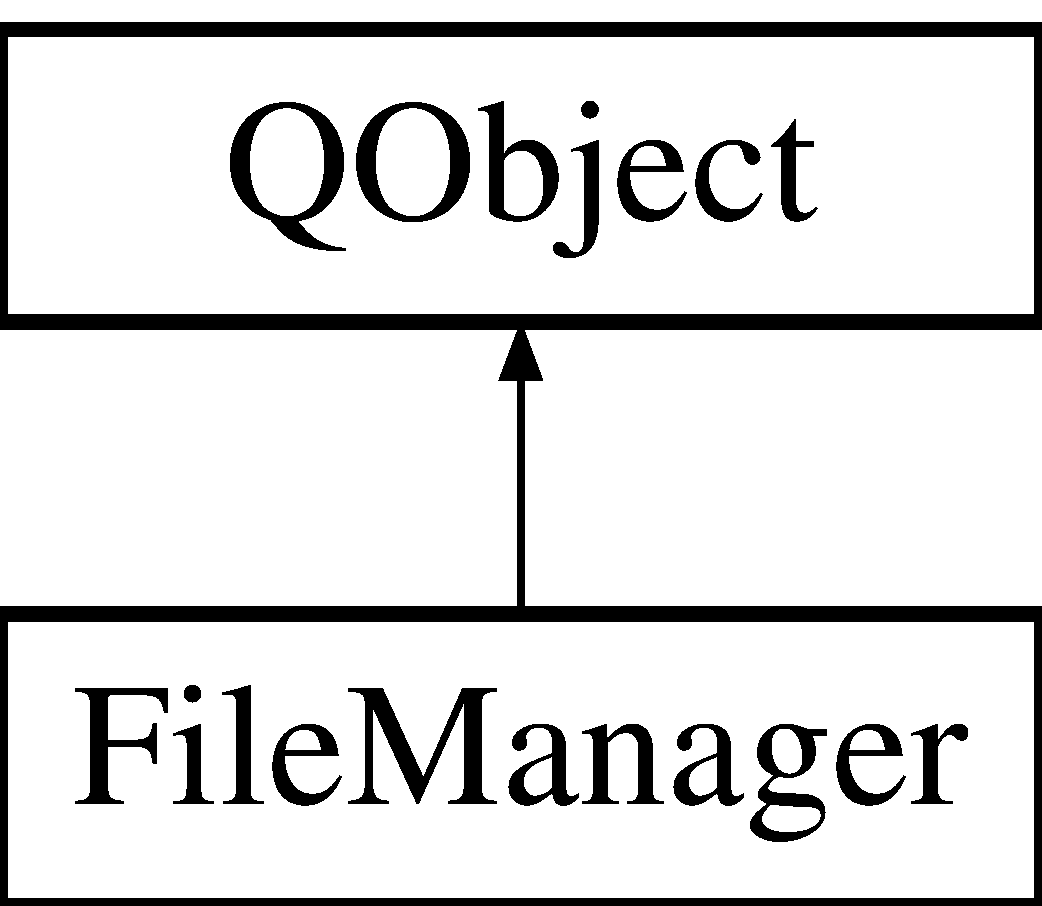
\includegraphics[height=2.000000cm]{class_file_manager}
\end{center}
\end{figure}
\subsection*{Public Member Functions}
\begin{DoxyCompactItemize}
\item 
\hyperlink{class_file_manager_aed06615dba6e3987ba4f129505e92edc}{File\+Manager} (Q\+Object $\ast$parent=0)
\item 
\hyperlink{class_file_manager_abaed33b5b0c13b8a597db9335a1aacfa}{$\sim$\+File\+Manager} ()
\item 
bool \hyperlink{class_file_manager_ac2f59a9eab9545d803729fd73438ff13}{read\+File} (const Q\+String \&file\+Name)
\item 
qint32 \hyperlink{class_file_manager_a152e84aab081c06a53abde7023ee341f}{get\+Processor\+Count} ()
\item 
qint32 \hyperlink{class_file_manager_a7bbda9c89953f666440a1550adf4bb2f}{parse\+File\+Contents} ()
\item 
Q\+String \& \hyperlink{class_file_manager_af6c82e156919875fb1bfbf3b6fc56c96}{get\+File\+Contents} ()
\end{DoxyCompactItemize}


\subsection{Constructor \& Destructor Documentation}
\mbox{\Hypertarget{class_file_manager_aed06615dba6e3987ba4f129505e92edc}\label{class_file_manager_aed06615dba6e3987ba4f129505e92edc}} 
\index{File\+Manager@{File\+Manager}!File\+Manager@{File\+Manager}}
\index{File\+Manager@{File\+Manager}!File\+Manager@{File\+Manager}}
\subsubsection{\texorpdfstring{File\+Manager()}{FileManager()}}
{\footnotesize\ttfamily File\+Manager\+::\+File\+Manager (\begin{DoxyParamCaption}\item[{Q\+Object $\ast$}]{parent = {\ttfamily 0} }\end{DoxyParamCaption})\hspace{0.3cm}{\ttfamily [explicit]}}

\mbox{\Hypertarget{class_file_manager_abaed33b5b0c13b8a597db9335a1aacfa}\label{class_file_manager_abaed33b5b0c13b8a597db9335a1aacfa}} 
\index{File\+Manager@{File\+Manager}!````~File\+Manager@{$\sim$\+File\+Manager}}
\index{````~File\+Manager@{$\sim$\+File\+Manager}!File\+Manager@{File\+Manager}}
\subsubsection{\texorpdfstring{$\sim$\+File\+Manager()}{~FileManager()}}
{\footnotesize\ttfamily File\+Manager\+::$\sim$\+File\+Manager (\begin{DoxyParamCaption}{ }\end{DoxyParamCaption})}



\subsection{Member Function Documentation}
\mbox{\Hypertarget{class_file_manager_af6c82e156919875fb1bfbf3b6fc56c96}\label{class_file_manager_af6c82e156919875fb1bfbf3b6fc56c96}} 
\index{File\+Manager@{File\+Manager}!get\+File\+Contents@{get\+File\+Contents}}
\index{get\+File\+Contents@{get\+File\+Contents}!File\+Manager@{File\+Manager}}
\subsubsection{\texorpdfstring{get\+File\+Contents()}{getFileContents()}}
{\footnotesize\ttfamily Q\+String \& File\+Manager\+::get\+File\+Contents (\begin{DoxyParamCaption}{ }\end{DoxyParamCaption})}

\mbox{\Hypertarget{class_file_manager_a152e84aab081c06a53abde7023ee341f}\label{class_file_manager_a152e84aab081c06a53abde7023ee341f}} 
\index{File\+Manager@{File\+Manager}!get\+Processor\+Count@{get\+Processor\+Count}}
\index{get\+Processor\+Count@{get\+Processor\+Count}!File\+Manager@{File\+Manager}}
\subsubsection{\texorpdfstring{get\+Processor\+Count()}{getProcessorCount()}}
{\footnotesize\ttfamily qint32 File\+Manager\+::get\+Processor\+Count (\begin{DoxyParamCaption}{ }\end{DoxyParamCaption})}

\mbox{\Hypertarget{class_file_manager_a7bbda9c89953f666440a1550adf4bb2f}\label{class_file_manager_a7bbda9c89953f666440a1550adf4bb2f}} 
\index{File\+Manager@{File\+Manager}!parse\+File\+Contents@{parse\+File\+Contents}}
\index{parse\+File\+Contents@{parse\+File\+Contents}!File\+Manager@{File\+Manager}}
\subsubsection{\texorpdfstring{parse\+File\+Contents()}{parseFileContents()}}
{\footnotesize\ttfamily qint32 File\+Manager\+::parse\+File\+Contents (\begin{DoxyParamCaption}{ }\end{DoxyParamCaption})}

\mbox{\Hypertarget{class_file_manager_ac2f59a9eab9545d803729fd73438ff13}\label{class_file_manager_ac2f59a9eab9545d803729fd73438ff13}} 
\index{File\+Manager@{File\+Manager}!read\+File@{read\+File}}
\index{read\+File@{read\+File}!File\+Manager@{File\+Manager}}
\subsubsection{\texorpdfstring{read\+File()}{readFile()}}
{\footnotesize\ttfamily bool File\+Manager\+::read\+File (\begin{DoxyParamCaption}\item[{const Q\+String \&}]{file\+Name }\end{DoxyParamCaption})}



The documentation for this class was generated from the following files\+:\begin{DoxyCompactItemize}
\item 
C\+:/\+Users/\+S\+H\+E\+K\+H\+A\+R/\+Desktop/\+C\+P\+U\+\_\+\+Info/\+C\+P\+U\+Information1/\hyperlink{filemanager_8h}{filemanager.\+h}\item 
C\+:/\+Users/\+S\+H\+E\+K\+H\+A\+R/\+Desktop/\+C\+P\+U\+\_\+\+Info/\+C\+P\+U\+Information1/\hyperlink{filemanager_8cpp}{filemanager.\+cpp}\end{DoxyCompactItemize}

\hypertarget{class_info_manager}{}\section{Info\+Manager Class Reference}
\label{class_info_manager}\index{Info\+Manager@{Info\+Manager}}


{\ttfamily \#include $<$infomanager.\+h$>$}

Inheritance diagram for Info\+Manager\+:\begin{figure}[H]
\begin{center}
\leavevmode
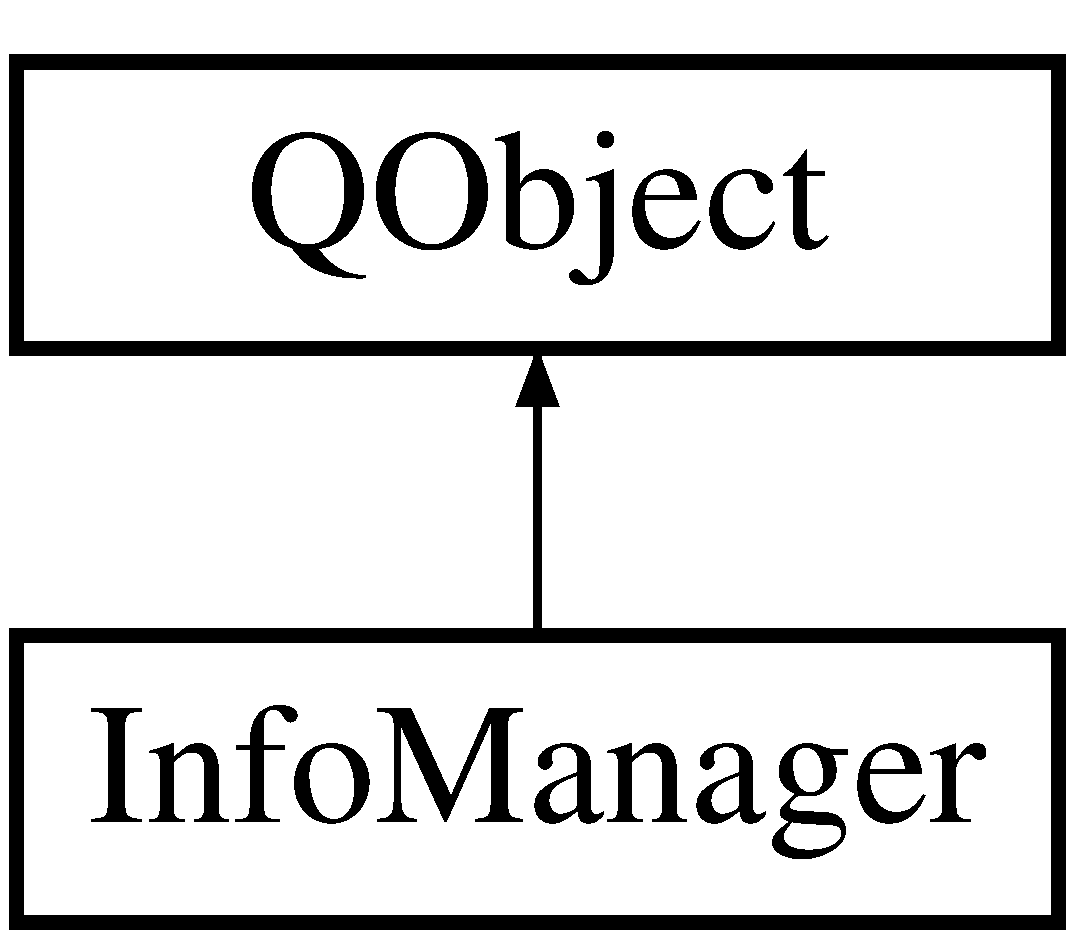
\includegraphics[height=2.000000cm]{class_info_manager}
\end{center}
\end{figure}
\subsection*{Public Member Functions}
\begin{DoxyCompactItemize}
\item 
\hyperlink{class_info_manager_abdddbbf624c1fb9a3815b1e720bca72a}{Info\+Manager} (Q\+Object $\ast$parent=0)
\item 
\hyperlink{class_info_manager_ae53b7e0f0a345170596d6e17198261bf}{$\sim$\+Info\+Manager} ()
\item 
void \hyperlink{class_info_manager_a13e29dc9ebb100b5ab8b640207f4401c}{parse\+C\+P\+U\+Raw\+Data} (qint32 processor\+Count, const Q\+String \&cpu\+Data)
\item 
Q\+List$<$ \hyperlink{class_c_p_u_info}{C\+P\+U\+Info} $\ast$ $>$ \hyperlink{class_info_manager_af5c7c292bc2e1b13b4ef8fb441b2ca2b}{get\+Processor\+List} ()
\end{DoxyCompactItemize}


\subsection{Constructor \& Destructor Documentation}
\mbox{\Hypertarget{class_info_manager_abdddbbf624c1fb9a3815b1e720bca72a}\label{class_info_manager_abdddbbf624c1fb9a3815b1e720bca72a}} 
\index{Info\+Manager@{Info\+Manager}!Info\+Manager@{Info\+Manager}}
\index{Info\+Manager@{Info\+Manager}!Info\+Manager@{Info\+Manager}}
\subsubsection{\texorpdfstring{Info\+Manager()}{InfoManager()}}
{\footnotesize\ttfamily Info\+Manager\+::\+Info\+Manager (\begin{DoxyParamCaption}\item[{Q\+Object $\ast$}]{parent = {\ttfamily 0} }\end{DoxyParamCaption})\hspace{0.3cm}{\ttfamily [explicit]}}

\mbox{\Hypertarget{class_info_manager_ae53b7e0f0a345170596d6e17198261bf}\label{class_info_manager_ae53b7e0f0a345170596d6e17198261bf}} 
\index{Info\+Manager@{Info\+Manager}!````~Info\+Manager@{$\sim$\+Info\+Manager}}
\index{````~Info\+Manager@{$\sim$\+Info\+Manager}!Info\+Manager@{Info\+Manager}}
\subsubsection{\texorpdfstring{$\sim$\+Info\+Manager()}{~InfoManager()}}
{\footnotesize\ttfamily Info\+Manager\+::$\sim$\+Info\+Manager (\begin{DoxyParamCaption}{ }\end{DoxyParamCaption})}



\subsection{Member Function Documentation}
\mbox{\Hypertarget{class_info_manager_af5c7c292bc2e1b13b4ef8fb441b2ca2b}\label{class_info_manager_af5c7c292bc2e1b13b4ef8fb441b2ca2b}} 
\index{Info\+Manager@{Info\+Manager}!get\+Processor\+List@{get\+Processor\+List}}
\index{get\+Processor\+List@{get\+Processor\+List}!Info\+Manager@{Info\+Manager}}
\subsubsection{\texorpdfstring{get\+Processor\+List()}{getProcessorList()}}
{\footnotesize\ttfamily Q\+List$<$ \hyperlink{class_c_p_u_info}{C\+P\+U\+Info} $\ast$ $>$ Info\+Manager\+::get\+Processor\+List (\begin{DoxyParamCaption}{ }\end{DoxyParamCaption})}

\mbox{\Hypertarget{class_info_manager_a13e29dc9ebb100b5ab8b640207f4401c}\label{class_info_manager_a13e29dc9ebb100b5ab8b640207f4401c}} 
\index{Info\+Manager@{Info\+Manager}!parse\+C\+P\+U\+Raw\+Data@{parse\+C\+P\+U\+Raw\+Data}}
\index{parse\+C\+P\+U\+Raw\+Data@{parse\+C\+P\+U\+Raw\+Data}!Info\+Manager@{Info\+Manager}}
\subsubsection{\texorpdfstring{parse\+C\+P\+U\+Raw\+Data()}{parseCPURawData()}}
{\footnotesize\ttfamily void Info\+Manager\+::parse\+C\+P\+U\+Raw\+Data (\begin{DoxyParamCaption}\item[{qint32}]{processor\+Count,  }\item[{const Q\+String \&}]{cpu\+Data }\end{DoxyParamCaption})}



The documentation for this class was generated from the following files\+:\begin{DoxyCompactItemize}
\item 
C\+:/\+Users/\+S\+H\+E\+K\+H\+A\+R/\+Desktop/\+C\+P\+U\+\_\+\+Info/\+C\+P\+U\+Information1/\hyperlink{infomanager_8h}{infomanager.\+h}\item 
C\+:/\+Users/\+S\+H\+E\+K\+H\+A\+R/\+Desktop/\+C\+P\+U\+\_\+\+Info/\+C\+P\+U\+Information1/\hyperlink{infomanager_8cpp}{infomanager.\+cpp}\end{DoxyCompactItemize}

\chapter{File Documentation}
\hypertarget{constantslist_8h}{}\section{C\+:/\+Users/\+S\+H\+E\+K\+H\+A\+R/\+Desktop/\+C\+P\+U\+\_\+\+Info/\+C\+P\+U\+Information1/constantslist.h File Reference}
\label{constantslist_8h}\index{C\+:/\+Users/\+S\+H\+E\+K\+H\+A\+R/\+Desktop/\+C\+P\+U\+\_\+\+Info/\+C\+P\+U\+Information1/constantslist.\+h@{C\+:/\+Users/\+S\+H\+E\+K\+H\+A\+R/\+Desktop/\+C\+P\+U\+\_\+\+Info/\+C\+P\+U\+Information1/constantslist.\+h}}
{\ttfamily \#include $<$Q\+String$>$}\newline
\subsection*{Variables}
\begin{DoxyCompactItemize}
\item 
const Q\+String \hyperlink{constantslist_8h_ac4815b6993a194e199cc210dc636655d}{Processsor\+Parameter} = \char`\"{}processor\char`\"{}
\item 
const Q\+String \hyperlink{constantslist_8h_af0e941688e091fd614a75ea8cd14787d}{Vendor\+Id} = \char`\"{}vendor\+\_\+id\char`\"{}
\item 
const Q\+String \hyperlink{constantslist_8h_a9c44ba5e3f6971ce1798771a8f2b6d1d}{C\+P\+U\+Family} = \char`\"{}cpu family\char`\"{}
\item 
const Q\+String \hyperlink{constantslist_8h_aaa5a824142d131af089081cbea376a9b}{Model} = \char`\"{}model\char`\"{}
\item 
const Q\+String \hyperlink{constantslist_8h_a2049c55c9afa9341d41ee396d667a2fb}{Model\+Name} = \char`\"{}model name\char`\"{}
\item 
const Q\+String \hyperlink{constantslist_8h_a28544f1f360e0f38bc889c76df87da64}{Stepping} = \char`\"{}stepping\char`\"{}
\item 
const Q\+String \hyperlink{constantslist_8h_aedde680dbaf85b85767bac811cced282}{Microcode} = \char`\"{}microcode\char`\"{}
\item 
const Q\+String \hyperlink{constantslist_8h_a30c23478810e3c2d0092428a9629292b}{C\+P\+U\+Frequency\+M\+Hz} = \char`\"{}cpu M\+Hz\char`\"{}
\end{DoxyCompactItemize}


\subsection{Variable Documentation}
\mbox{\Hypertarget{constantslist_8h_a9c44ba5e3f6971ce1798771a8f2b6d1d}\label{constantslist_8h_a9c44ba5e3f6971ce1798771a8f2b6d1d}} 
\index{constantslist.\+h@{constantslist.\+h}!C\+P\+U\+Family@{C\+P\+U\+Family}}
\index{C\+P\+U\+Family@{C\+P\+U\+Family}!constantslist.\+h@{constantslist.\+h}}
\subsubsection{\texorpdfstring{C\+P\+U\+Family}{CPUFamily}}
{\footnotesize\ttfamily const Q\+String C\+P\+U\+Family = \char`\"{}cpu family\char`\"{}}

\mbox{\Hypertarget{constantslist_8h_a30c23478810e3c2d0092428a9629292b}\label{constantslist_8h_a30c23478810e3c2d0092428a9629292b}} 
\index{constantslist.\+h@{constantslist.\+h}!C\+P\+U\+Frequency\+M\+Hz@{C\+P\+U\+Frequency\+M\+Hz}}
\index{C\+P\+U\+Frequency\+M\+Hz@{C\+P\+U\+Frequency\+M\+Hz}!constantslist.\+h@{constantslist.\+h}}
\subsubsection{\texorpdfstring{C\+P\+U\+Frequency\+M\+Hz}{CPUFrequencyMHz}}
{\footnotesize\ttfamily const Q\+String C\+P\+U\+Frequency\+M\+Hz = \char`\"{}cpu M\+Hz\char`\"{}}

\mbox{\Hypertarget{constantslist_8h_aedde680dbaf85b85767bac811cced282}\label{constantslist_8h_aedde680dbaf85b85767bac811cced282}} 
\index{constantslist.\+h@{constantslist.\+h}!Microcode@{Microcode}}
\index{Microcode@{Microcode}!constantslist.\+h@{constantslist.\+h}}
\subsubsection{\texorpdfstring{Microcode}{Microcode}}
{\footnotesize\ttfamily const Q\+String Microcode = \char`\"{}microcode\char`\"{}}

\mbox{\Hypertarget{constantslist_8h_aaa5a824142d131af089081cbea376a9b}\label{constantslist_8h_aaa5a824142d131af089081cbea376a9b}} 
\index{constantslist.\+h@{constantslist.\+h}!Model@{Model}}
\index{Model@{Model}!constantslist.\+h@{constantslist.\+h}}
\subsubsection{\texorpdfstring{Model}{Model}}
{\footnotesize\ttfamily const Q\+String Model = \char`\"{}model\char`\"{}}

\mbox{\Hypertarget{constantslist_8h_a2049c55c9afa9341d41ee396d667a2fb}\label{constantslist_8h_a2049c55c9afa9341d41ee396d667a2fb}} 
\index{constantslist.\+h@{constantslist.\+h}!Model\+Name@{Model\+Name}}
\index{Model\+Name@{Model\+Name}!constantslist.\+h@{constantslist.\+h}}
\subsubsection{\texorpdfstring{Model\+Name}{ModelName}}
{\footnotesize\ttfamily const Q\+String Model\+Name = \char`\"{}model name\char`\"{}}

\mbox{\Hypertarget{constantslist_8h_ac4815b6993a194e199cc210dc636655d}\label{constantslist_8h_ac4815b6993a194e199cc210dc636655d}} 
\index{constantslist.\+h@{constantslist.\+h}!Processsor\+Parameter@{Processsor\+Parameter}}
\index{Processsor\+Parameter@{Processsor\+Parameter}!constantslist.\+h@{constantslist.\+h}}
\subsubsection{\texorpdfstring{Processsor\+Parameter}{ProcesssorParameter}}
{\footnotesize\ttfamily const Q\+String Processsor\+Parameter = \char`\"{}processor\char`\"{}}

\mbox{\Hypertarget{constantslist_8h_a28544f1f360e0f38bc889c76df87da64}\label{constantslist_8h_a28544f1f360e0f38bc889c76df87da64}} 
\index{constantslist.\+h@{constantslist.\+h}!Stepping@{Stepping}}
\index{Stepping@{Stepping}!constantslist.\+h@{constantslist.\+h}}
\subsubsection{\texorpdfstring{Stepping}{Stepping}}
{\footnotesize\ttfamily const Q\+String Stepping = \char`\"{}stepping\char`\"{}}

\mbox{\Hypertarget{constantslist_8h_af0e941688e091fd614a75ea8cd14787d}\label{constantslist_8h_af0e941688e091fd614a75ea8cd14787d}} 
\index{constantslist.\+h@{constantslist.\+h}!Vendor\+Id@{Vendor\+Id}}
\index{Vendor\+Id@{Vendor\+Id}!constantslist.\+h@{constantslist.\+h}}
\subsubsection{\texorpdfstring{Vendor\+Id}{VendorId}}
{\footnotesize\ttfamily const Q\+String Vendor\+Id = \char`\"{}vendor\+\_\+id\char`\"{}}


\hypertarget{cpuinfo_8cpp}{}\section{C\+:/\+Users/\+S\+H\+E\+K\+H\+A\+R/\+Desktop/\+C\+P\+U\+\_\+\+Info/\+C\+P\+U\+Information1/cpuinfo.cpp File Reference}
\label{cpuinfo_8cpp}\index{C\+:/\+Users/\+S\+H\+E\+K\+H\+A\+R/\+Desktop/\+C\+P\+U\+\_\+\+Info/\+C\+P\+U\+Information1/cpuinfo.\+cpp@{C\+:/\+Users/\+S\+H\+E\+K\+H\+A\+R/\+Desktop/\+C\+P\+U\+\_\+\+Info/\+C\+P\+U\+Information1/cpuinfo.\+cpp}}
{\ttfamily \#include \char`\"{}cpuinfo.\+h\char`\"{}}\newline

\hypertarget{cpuinfo_8h}{}\section{C\+:/\+Users/\+S\+H\+E\+K\+H\+A\+R/\+Desktop/\+C\+P\+U\+\_\+\+Info/\+C\+P\+U\+Information1/cpuinfo.h File Reference}
\label{cpuinfo_8h}\index{C\+:/\+Users/\+S\+H\+E\+K\+H\+A\+R/\+Desktop/\+C\+P\+U\+\_\+\+Info/\+C\+P\+U\+Information1/cpuinfo.\+h@{C\+:/\+Users/\+S\+H\+E\+K\+H\+A\+R/\+Desktop/\+C\+P\+U\+\_\+\+Info/\+C\+P\+U\+Information1/cpuinfo.\+h}}
{\ttfamily \#include $<$Q\+Object$>$}\newline
{\ttfamily \#include $<$Q\+String\+List$>$}\newline
\subsection*{Classes}
\begin{DoxyCompactItemize}
\item 
class \hyperlink{class_c_p_u_info}{C\+P\+U\+Info}
\end{DoxyCompactItemize}

\hypertarget{cpulist_8cpp}{}\section{C\+:/\+Users/\+S\+H\+E\+K\+H\+A\+R/\+Desktop/\+C\+P\+U\+\_\+\+Info/\+C\+P\+U\+Information1/cpulist.cpp File Reference}
\label{cpulist_8cpp}\index{C\+:/\+Users/\+S\+H\+E\+K\+H\+A\+R/\+Desktop/\+C\+P\+U\+\_\+\+Info/\+C\+P\+U\+Information1/cpulist.\+cpp@{C\+:/\+Users/\+S\+H\+E\+K\+H\+A\+R/\+Desktop/\+C\+P\+U\+\_\+\+Info/\+C\+P\+U\+Information1/cpulist.\+cpp}}
{\ttfamily \#include \char`\"{}cpulist.\+h\char`\"{}}\newline

\hypertarget{cpulist_8h}{}\section{C\+:/\+Users/\+S\+H\+E\+K\+H\+A\+R/\+Desktop/\+C\+P\+U\+\_\+\+Info/\+C\+P\+U\+Information1/cpulist.h File Reference}
\label{cpulist_8h}\index{C\+:/\+Users/\+S\+H\+E\+K\+H\+A\+R/\+Desktop/\+C\+P\+U\+\_\+\+Info/\+C\+P\+U\+Information1/cpulist.\+h@{C\+:/\+Users/\+S\+H\+E\+K\+H\+A\+R/\+Desktop/\+C\+P\+U\+\_\+\+Info/\+C\+P\+U\+Information1/cpulist.\+h}}
{\ttfamily \#include \char`\"{}cpuinfo.\+h\char`\"{}}\newline
{\ttfamily \#include $<$Q\+Object$>$}\newline
{\ttfamily \#include $<$Q\+List$>$}\newline
{\ttfamily \#include $<$Q\+Qml\+List\+Property$>$}\newline
\subsection*{Classes}
\begin{DoxyCompactItemize}
\item 
class \hyperlink{class_c_p_u_list}{C\+P\+U\+List}
\end{DoxyCompactItemize}

\hypertarget{filemanager_8cpp}{}\section{C\+:/\+Users/\+S\+H\+E\+K\+H\+A\+R/\+Desktop/\+C\+P\+U\+\_\+\+Info/\+C\+P\+U\+Information1/filemanager.cpp File Reference}
\label{filemanager_8cpp}\index{C\+:/\+Users/\+S\+H\+E\+K\+H\+A\+R/\+Desktop/\+C\+P\+U\+\_\+\+Info/\+C\+P\+U\+Information1/filemanager.\+cpp@{C\+:/\+Users/\+S\+H\+E\+K\+H\+A\+R/\+Desktop/\+C\+P\+U\+\_\+\+Info/\+C\+P\+U\+Information1/filemanager.\+cpp}}
{\ttfamily \#include \char`\"{}filemanager.\+h\char`\"{}}\newline
{\ttfamily \#include \char`\"{}constantslist.\+h\char`\"{}}\newline
{\ttfamily \#include $<$Q\+Object$>$}\newline
{\ttfamily \#include $<$Q\+File$>$}\newline
{\ttfamily \#include $<$Q\+Text\+Stream$>$}\newline
{\ttfamily \#include $<$Q\+Message\+Box$>$}\newline
{\ttfamily \#include $<$Q\+Debug$>$}\newline

\hypertarget{filemanager_8h}{}\section{C\+:/\+Users/\+S\+H\+E\+K\+H\+A\+R/\+Desktop/\+C\+P\+U\+\_\+\+Info/\+C\+P\+U\+Information1/filemanager.h File Reference}
\label{filemanager_8h}\index{C\+:/\+Users/\+S\+H\+E\+K\+H\+A\+R/\+Desktop/\+C\+P\+U\+\_\+\+Info/\+C\+P\+U\+Information1/filemanager.\+h@{C\+:/\+Users/\+S\+H\+E\+K\+H\+A\+R/\+Desktop/\+C\+P\+U\+\_\+\+Info/\+C\+P\+U\+Information1/filemanager.\+h}}
{\ttfamily \#include $<$Q\+Object$>$}\newline
\subsection*{Classes}
\begin{DoxyCompactItemize}
\item 
class \hyperlink{class_file_manager}{File\+Manager}
\end{DoxyCompactItemize}

\hypertarget{infomanager_8cpp}{}\section{C\+:/\+Users/\+S\+H\+E\+K\+H\+A\+R/\+Desktop/\+C\+P\+U\+\_\+\+Info/\+C\+P\+U\+Information1/infomanager.cpp File Reference}
\label{infomanager_8cpp}\index{C\+:/\+Users/\+S\+H\+E\+K\+H\+A\+R/\+Desktop/\+C\+P\+U\+\_\+\+Info/\+C\+P\+U\+Information1/infomanager.\+cpp@{C\+:/\+Users/\+S\+H\+E\+K\+H\+A\+R/\+Desktop/\+C\+P\+U\+\_\+\+Info/\+C\+P\+U\+Information1/infomanager.\+cpp}}
{\ttfamily \#include \char`\"{}infomanager.\+h\char`\"{}}\newline
{\ttfamily \#include \char`\"{}constantslist.\+h\char`\"{}}\newline
{\ttfamily \#include $<$Q\+Debug$>$}\newline

\hypertarget{infomanager_8h}{}\section{C\+:/\+Users/\+S\+H\+E\+K\+H\+A\+R/\+Desktop/\+C\+P\+U\+\_\+\+Info/\+C\+P\+U\+Information1/infomanager.h File Reference}
\label{infomanager_8h}\index{C\+:/\+Users/\+S\+H\+E\+K\+H\+A\+R/\+Desktop/\+C\+P\+U\+\_\+\+Info/\+C\+P\+U\+Information1/infomanager.\+h@{C\+:/\+Users/\+S\+H\+E\+K\+H\+A\+R/\+Desktop/\+C\+P\+U\+\_\+\+Info/\+C\+P\+U\+Information1/infomanager.\+h}}
{\ttfamily \#include \char`\"{}cpuinfo.\+h\char`\"{}}\newline
{\ttfamily \#include $<$Q\+Object$>$}\newline
{\ttfamily \#include $<$Q\+List$>$}\newline
\subsection*{Classes}
\begin{DoxyCompactItemize}
\item 
class \hyperlink{class_info_manager}{Info\+Manager}
\end{DoxyCompactItemize}

\hypertarget{main_8cpp}{}\section{C\+:/\+Users/\+S\+H\+E\+K\+H\+A\+R/\+Desktop/\+C\+P\+U\+\_\+\+Info/\+C\+P\+U\+Information1/main.cpp File Reference}
\label{main_8cpp}\index{C\+:/\+Users/\+S\+H\+E\+K\+H\+A\+R/\+Desktop/\+C\+P\+U\+\_\+\+Info/\+C\+P\+U\+Information1/main.\+cpp@{C\+:/\+Users/\+S\+H\+E\+K\+H\+A\+R/\+Desktop/\+C\+P\+U\+\_\+\+Info/\+C\+P\+U\+Information1/main.\+cpp}}
{\ttfamily \#include $<$Q\+Gui\+Application$>$}\newline
{\ttfamily \#include $<$Q\+Qml\+Application\+Engine$>$}\newline
{\ttfamily \#include $<$Q\+Qml\+Context$>$}\newline
{\ttfamily \#include $<$Q\+Quick\+View$>$}\newline
{\ttfamily \#include $<$Q\+Qml\+Component$>$}\newline
{\ttfamily \#include \char`\"{}filemanager.\+h\char`\"{}}\newline
{\ttfamily \#include \char`\"{}infomanager.\+h\char`\"{}}\newline
{\ttfamily \#include \char`\"{}cpulist.\+h\char`\"{}}\newline
\subsection*{Functions}
\begin{DoxyCompactItemize}
\item 
int \hyperlink{main_8cpp_a0ddf1224851353fc92bfbff6f499fa97}{main} (int argc, char $\ast$argv\mbox{[}$\,$\mbox{]})
\end{DoxyCompactItemize}


\subsection{Function Documentation}
\mbox{\Hypertarget{main_8cpp_a0ddf1224851353fc92bfbff6f499fa97}\label{main_8cpp_a0ddf1224851353fc92bfbff6f499fa97}} 
\index{main.\+cpp@{main.\+cpp}!main@{main}}
\index{main@{main}!main.\+cpp@{main.\+cpp}}
\subsubsection{\texorpdfstring{main()}{main()}}
{\footnotesize\ttfamily int main (\begin{DoxyParamCaption}\item[{int}]{argc,  }\item[{char $\ast$}]{argv\mbox{[}$\,$\mbox{]} }\end{DoxyParamCaption})}

\mbox{[}register list\mbox{]}

\mbox{[}register list\mbox{]}
%--- End generated contents ---

% Index
\backmatter
\newpage
\phantomsection
\clearemptydoublepage
\addcontentsline{toc}{chapter}{Index}
\printindex

\end{document}
